\section{Análise complementar dos resultados sintéticos}
\label{sec:posthoc}

As previsões por trajetória foram recalculadas a partir dos checkpoints
congelados (diferença relativa máxima de $10^{-8}$ em relação ao MSE reportado),
sem retreino e sem alterar o protocolo. Como os parâmetros têm escalas
diferentes, cada erro quadrático é dividido pela variância do parâmetro no
conjunto de treino; o resultado complementar é o $R^2$ em relação ao
estimador trivial que sempre prevê a média a priori.

\begin{table}[htbp]
\centering
\caption{$R^2$ por parâmetro em relação à média a priori, erro absoluto
mediano macro e MSE da razão de ramificação no teste sintético.}
\label{tab:posthoc-r2}
\small
\begin{tabular}{lrrrrrr}
\toprule
Estimador & $\mu$ & $\alpha_{\mathrm{self}}$ & $\alpha_{\mathrm{cross}}$ & $\beta$ & EA mediano & MSE de $g$\\
\midrule
Média a priori & $-$0,01 & 0,00 & $-$0,01 & 0,01 & 0,1908 & 0,0670\\
MLE & 0,24 & 0,90 & 0,90 & $-$15,64 & 0,0674 & 0,0023\\
LSTM (ensemble) & 0,84 & 0,82 & 0,81 & 0,65 & 0,0680 & 0,0017\\
Transformer (ensemble) & 0,84 & 0,74 & 0,73 & 0,61 & 0,0765 & 0,0019\\
\bottomrule
\end{tabular}
\end{table}

\begin{table}[htbp]
\centering
\caption{Comparação pareada por trajetória (erro quadrático padronizado médio
nos quatro parâmetros). Colunas: perda mediana de A e de B, fração de
trajetórias em que A erra menos e IC 95\% \emph{bootstrap} da diferença média
A$-$B (negativo favorece A).}
\label{tab:posthoc-pareado}
\footnotesize
\begin{tabular}{llrrrr}
\toprule
A $\times$ B & Regime & Med.\ A & Med.\ B & A melhor & IC 95\% (A$-$B)\\
\midrule
LSTM $\times$ Transformer & todos & 0,151 & 0,187 & 70,2\% & [$-$0,051; $-$0,047]\\
LSTM $\times$ Transformer & $g$ baixo & 0,112 & 0,131 & 61,1\% & [$-$0,021; $-$0,016]\\
LSTM $\times$ Transformer & $g$ intermediário & 0,127 & 0,164 & 72,8\% & [$-$0,045; $-$0,041]\\
LSTM $\times$ Transformer & $g$ quase crítico & 0,237 & 0,304 & 76,7\% & [$-$0,089; $-$0,081]\\
\midrule
LSTM $\times$ MLE & todos & 0,151 & 0,149 & 48,8\% & [$-$9,394; $-$0,809]\\
LSTM $\times$ MLE & $g$ baixo & 0,112 & 0,199 & 63,5\% & [$-$26,977; $-$2,225]\\
LSTM $\times$ MLE & $g$ intermediário & 0,127 & 0,100 & 40,1\% & [$-$0,040; $-$0,009]\\
LSTM $\times$ MLE & $g$ quase crítico & 0,237 & 0,183 & 42,7\% & [$-$0,467; $-$0,277]\\
\midrule
Transformer $\times$ MLE & todos & 0,187 & 0,149 & 43,5\% & [$-$9,376; $-$0,782]\\
Transformer $\times$ MLE & $g$ baixo & 0,131 & 0,199 & 59,4\% & [$-$27,686; $-$2,207]\\
Transformer $\times$ MLE & $g$ intermediário & 0,164 & 0,100 & 34,2\% & [0,002; 0,035]\\
Transformer $\times$ MLE & $g$ quase crítico & 0,304 & 0,183 & 36,7\% & [$-$0,374; $-$0,195]\\
\bottomrule
\end{tabular}
\end{table}

Primeiro, a vantagem das redes sobre
o MLE no MSE agregado vem de poucas trajetórias: 94,4\% da soma
dos erros quadráticos de $\beta$ do MLE se concentra em 1\% das trajetórias,
quase todas no regime de $g$ baixo. Em todas as 300 piores, a log-verossimilhança
no estimador supera a do parâmetro verdadeiro (ganho mediano de 2,80), e reajustar
100 delas com 20 inícios praticamente não altera o resultado. Não é
falha numérica: com excitação fraca, $\beta$ é pouco identificado em 1.000
eventos. Segundo, na trajetória típica o MLE é tão bom quanto as redes ou
melhor: a perda mediana é praticamente igual à da LSTM no agregado e menor nos
regimes intermediário e quase crítico. Terceiro, na comparação pareada o
ensemble LSTM supera o ensemble Transformer em todos os regimes; entre seeds
isoladas, contudo, a diferença não é significativa (Welch, $p=0,19$;
Mann--Whitney, $p=0,056$), porque a LSTM
apresentou dois níveis de convergência entre seeds.

\begin{figure}[htbp]
\centering
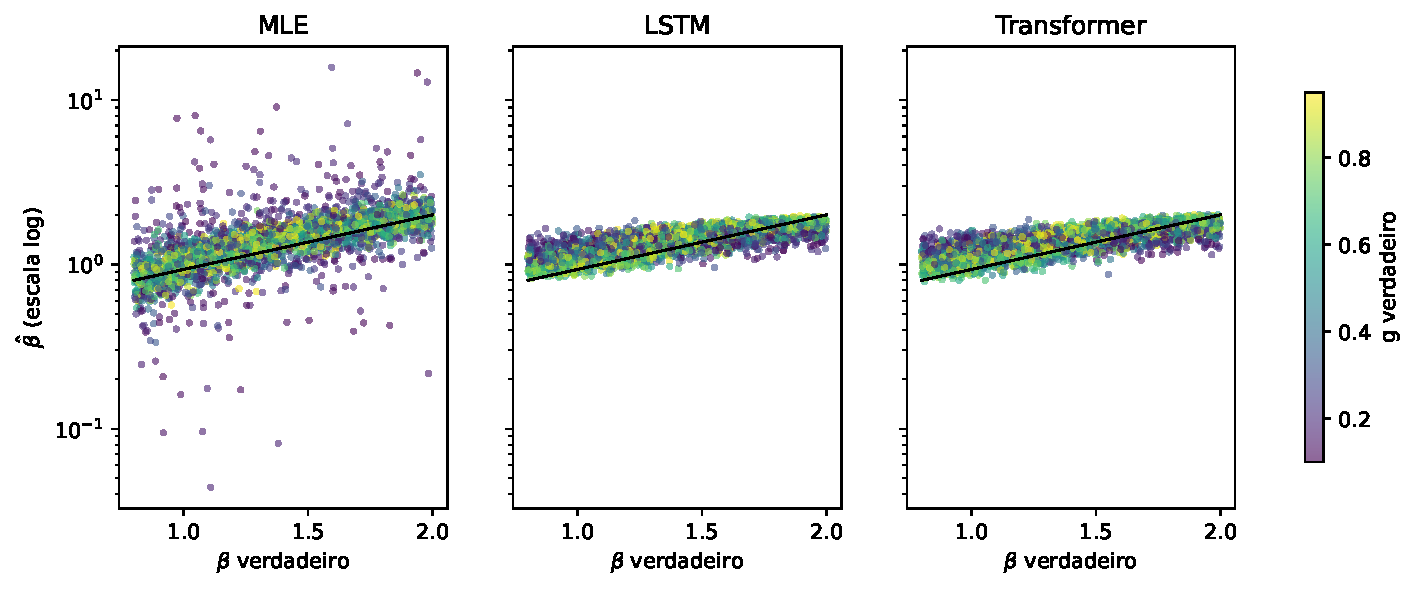
\includegraphics[width=0.95\linewidth]{../build/figures/posthoc_beta_verdadeiro_vs_estimado.pdf}
\caption{$\beta$ verdadeiro versus estimado (3.000 trajetórias de teste,
escala logarítmica). As redes encolhem as estimativas para o centro do
prior; o MLE é não viesado na maior parte do domínio, mas produz valores
extremos quando $g$ é baixo.}
\label{fig:posthoc-beta}
\end{figure}

\section{Calibração empírica e suporte do prior sintético}
\label{sec:calibracao}

O MLE foi ajustado nas 1063 janelas de 1.000 eventos do
bloco \texttt{calibration\_train} (15 a 22 de janeiro de 2024), único bloco
autorizado para calibração. A mediana de $\beta$ foi 2,71 (intervalo
interquartil 2,21--3,14), acima do limite de 2,0 usado no treino, e
$\alpha_{\mathrm{cross}}$ ficou abaixo de $10^{-3}$ em 89,4\% das janelas.
Apenas 15,4\% das janelas têm $\beta$ dentro do
prior, 0,4\% têm a fração autoexcitada
dentro de $[0{,}2;\,0{,}8]$ e 0,0\% satisfazem
todas as faixas ao mesmo tempo. Como um estimador treinado com perda
quadrática aproxima a média a posteriori sob o prior de treino, as redes
atuais não podem produzir estimativas nessa região; a avaliação empírica
exige recalibrar o prior ou treinar com rótulos MLE em janelas reais.

\begin{figure}[htbp]
\centering
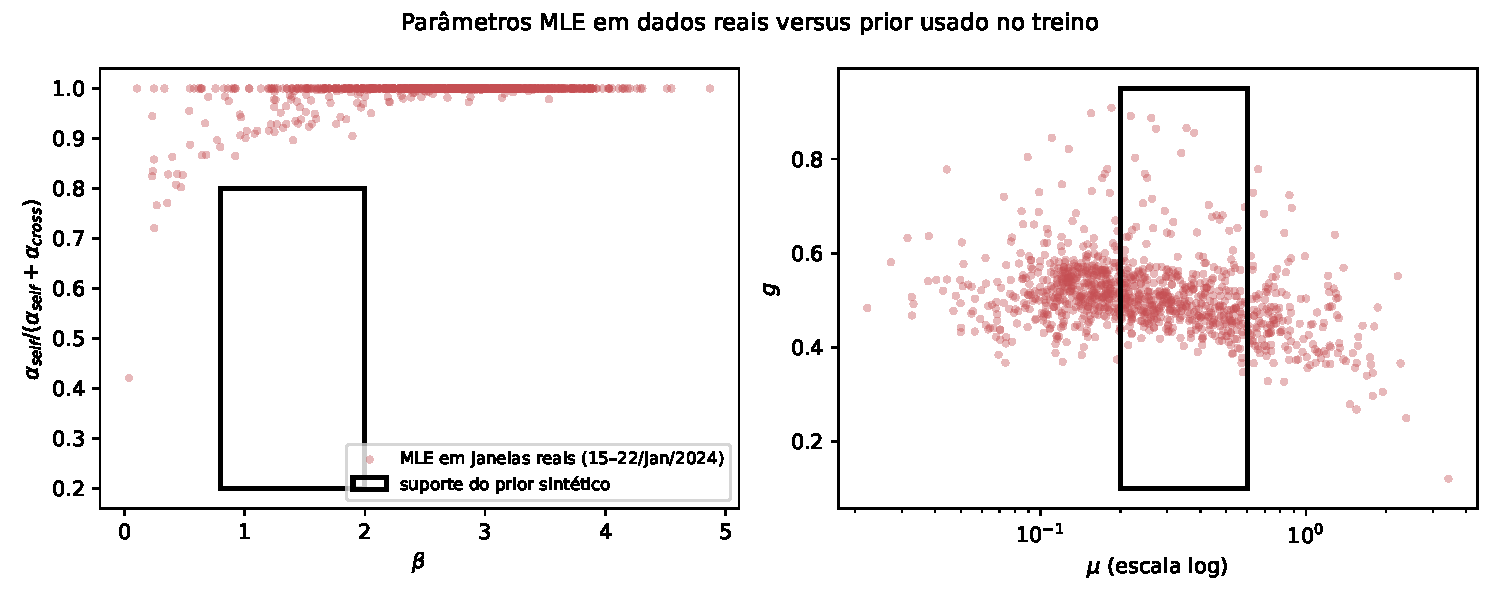
\includegraphics[width=0.95\linewidth]{../build/figures/posthoc_calibracao_vs_prior.pdf}
\caption{Estimativas MLE nas janelas reais de calibração (pontos) e suporte
do prior usado para gerar os dados de treino (retângulos).}
\label{fig:calibracao-prior}
\end{figure}
